% Lorentz.tex      pdflatex ZhCvGo15
% Diffuse globally, compute locally: a cyclist tale
% Tingnan Zhang, Daniel I. Goldman and Predrag Cvitanovi\'c

%\section{Diffusion in periodic arrays}
%\label{s-Lorentz}

\begin{figure}[htbp]
  \begin{center}
    (a)\;\includegraphics[width=0.43\textwidth]{diffuseSchreiberFig1}
    (b)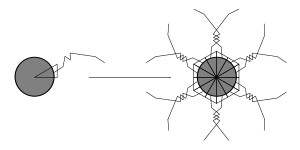
\includegraphics[width=0.45\textwidth]{diffuseSchreiberFig2}
  \end{center}
  \caption[]{\label{fig-schrieberFig12}
  (a) Motion in the fundamental domain (top left), elementary cell (top
      right) and the full space (bottom).
  (b) The above trajectory unwrapped in the full space and its 12 copies
    obtained by applying all point group \Dn{6} actions to it (from
    \refref{CGS92}).
  }
\end{figure}

For any dynamical system that has
translational symmetry, the full {\statesp} $\hM$ (\ie, both spatial
coordinates and momenta) has a periodic tiling
\[ %beq
\hM=\bigcup_{ \hn \in T} \pS_{\hn},
\] %eeq
by {\em translating} $\pS_{\hn}$ of an {\em elementary cell} $\pS$,
with $T$ the abelian group of lattice translations.

\begin{figure}[htbp]
	\begin{center}
    \includegraphics[width=0.25\textwidth]{diffuseLorentzGasParams}
	\end{center}
	\caption[]{\label{fig-LorentzGasParams}
        An elementary cell and its six unit translations. The ratio of
        distance $w$ between the nearest pair of disks to the    disk
        radius $r$ determines the dynamical properties in the system.
	}
	\TZ{2016-01-15}{This figure is also generated by me.}
\end{figure}

In the context of the triangular Lorentz gas system, an elementary
cell is the hexagon centered at a scatterer and lattice translations
$T$ applys only to spatial degrees of freedom, see
\reffig{fig-LorentzGasParams}. The dynamics restricted inside the
elementary cell is treated as the periodic boundary condition: when
the particle leaves the edge of the hexagon cell, it immediately
enters the region again from the opposite edge. The transition between
the finite and the infinite horizon is controlled by the ratio of $w/r$,
where $w$ is the gap between nearest pair of disk and $r$ the radius
of the disk. The horizon is finite for $w/r < 4/\sqrt{3}-2 =
0.3094\dots$.

When this elementary cell is itself invariant under a discrete symmetry
group $G$ the lattice can be tiled into images under $G$ and the lattice
translations of a fundamental domain.

When, in addition to translational invariance, the elementary cell is
invariant under a discrete symmetry group (point group) $G$, the
lattice can be tiled into images under $G$ and the lattice
translations of a fundamental domain.

Parenthetically, much of the literature, such as Bunimovich and Sinai\rf{BunSin81},
is focused only on the group of discrete translations, and what they
refer to as ``fundamental domain'' is here called ``elementary cell.''

The symmetry of the triangular periodic Lorentz gas is the space group
$p6mm$ (see Cotton\rf{Cotton08} {\em Chemical applications of group
theory},  Chapt.~11, for a pretty discussion of the geometry of space
groups). Space group $p6mm$ has a point subgroup $C_{6v}=\Dn{6}$.
Leaving the mathematical representation of group for later discussion,
we can intuitively understand the symmetry by decomposing the
hexagonal elementary cell into 12 identical triangular tiles, as in
\reffig{fig-schrieberFig12}\,(a), upper left, the fundamental domain
and its 11 copies. The fundamental domain tiles the full hexagon, by
application of the \Dn{6} rotations around the center or reflection
along symmetry lines, \ie, the point group actions.


Because we will work with different
kinds of \statesp s, through out the text we will repeatedly using tildes
($\tilde{\quad}$), nothings and hats ($\hat{\quad}$) atop symbols to
signify the dynamical quantities in the fundamental domain, elementary
cell and full {\statesp}, respectively.

As we will work with three kinds of \statesp s, we state here what
tildes, nothings and hats atop symbols signify:
\bea
\tilde{\ }     &~~&
    \mbox{fundamental domain, triangle in \reffig{fig-schrieberFig12}}
        \continue
%[nothing] \qquad \qquad &&
[0pt] \qquad \qquad &&
    \mbox{elementary cell, hexagon in \reffig{fig-schrieberFig12}}
        \continue
\hat{\ }   &&
    \mbox{full {\statesp}, lattice in \reffig{fig-schrieberFig12}}
\label{atops}
\eea

In addition to the full space and elementary cell \evOper\ , we denote
the quantity $\tx(t)\,=\,\tflow{t}{\tx}$ as the flow in the
fundamental domain ${\widetilde \pS}$. $\tflow{t}{\tx}$ is related to
$\flow{t}{\tx}$ by a discrete symmetry $g \in G$ which maps $\tx(t)\in
{\widetilde \pS}$ to ${x}(t) \in {\pS}$.

We have shown in \refsect{s-POT} that, for the
dynamics in the elementary cell, the displacement traveled along a
cycle is independent of the starting point. When we take into account
the point group symmetry (\ie, rotations and reflections), the above
statement does  not stand. While a full space (or elementary cell)
trajectory can be uniquely reduced to its fundamental domain counter
part by wrapping (reflecting and rotating) all the individual segments
in different fundamental domain into a single one, the reverse process
is always one-to-many. Because the fundamental domain does not have the
concepts of absolute orientation, a single unwrapped trajectory may
have up-to 12 isometric copies after we apply the discrete group
actions. Even worse, depending on where we start to unwrap the
trajectory, the full space trajectories can be completely different in
shape. A precise mathematical treatment is necessary to address the
above effects, before we can proceed to the complete formula for
diffusion, which depends on descriptions of displacements.


\bigskip
=========== TO REUSE ========

    \PC{2015-10-21}
    {edits based Cvitanovi\'c,  Eckmann,and Gaspard\rf{LorentzDiff}}
The lattice symmetry of the Lorentz billiard has important consequence on
the properties of the function $Q(\beta)$ are best illustrated by
introducing its analytic continuation at $\beta = i k$.  The function
$F(k)=Q(ik)$ is the rate associated with the incoherent scattering
function $\langle \exp i k \cdot (\hat x_t - x) \rangle_M$ considered in
light or neutron scattering experiments in liquids, in particular, by Van
Hove\rf{BoonYip80,VanHove54}. The vector $k$ is interpreted as the
wavenumber of the hydrodynamic modes of diffusion which we also find in
the Lorentz gas.  The function $F(k)$ turns out to be a dispersion
relation since $F(k)=-D k^2 + {\cal O}(k^4)$ in an isotropic diffusive
system.  The isotropy of a liquid implies that the dispersion relation
only depends on the amplitude $\vert k\vert$ of the wavenumber.


On the other hand, the lattice symmetry of the Lorentz gas
imposes special restrictions on the properties of the dispersion relation
$F(k)$ and on the values taken by the wavenumber.  The present classical
problem of diffusion is similar to the quantum motion of a particle in a
periodic potential.  Hence, the wavenumber takes its values in the so-called
Brillouin zone\rf{BoSmWi36,Harrison70}.  A mode of diffusion is associated with each value of
the wavenumber $k$ so that the direction of $k$ is privileged in the
system.  As a consequence, the symmetry of the lattice is reduced by the choice
of $k$.  This symmetry reduction is formalized by the concept of little group
associated with the wavenumber $k$, which is the subgroup of the lattice point
group leaving invariant the vector $k$.  For most values of $k$ inside the
Brillouin zone, the little group is trivial because it contains only the
identity.  However, the little group is larger when the wavenumber belongs to
special symmetry lines or symmetry points in the Brillouin zone.  In particular,
the little group coincides with the full point group when $k=0$.

The preceding considerations concern the consequences of the lattice symmetry
on the factorization of the zeta function.  There is a different problem which
is to express the zeta function in terms of the prime \po s of the
fundamental domain $\tilde M$ of the lattice (see Fig. 2) rather than
those of the elementary (Wigner-Seitz) cell $M$.
%This problem is a priori independent of the factorization
%discussed above and presents the following difficulty.
Here the stumbling block appears to be
the breaking of the rotational symmetry by
the auxilliary vector $\beta$, or, in other words,
the non-commutativity of translations and rotations.
More precisely, the global distance
$ \hat\phi^{r \period{\tilde{p}}} (\tx{\tpk}) - \tx{\tpk} $, $\tx{\tpk} \in \tp$,
% $ \hn_{r |\t p|}(\tx{\tpk}) $
depends on the starting cycle point if
$\tp$ is only a segment of the global cycle $p$. An
example is the diamond-shaped cycle of Fig.~3;
%the problem is that the $\tp$ segment of
%the global trajectory is not a translation in $\hM$.
depending whether one starts at $\tx_1$ or $\tx_2$, the global
distance covered in time $\period{\tilde{p}}$ is either the short or the
long diagonal.

In triangular and square lattices the diffusion is isotropic, but the
full function $Q(\beta)$ contains more information on the lattice
symmetry than the diffusion matrix of the second derivatives of
$Q(\beta)$. The behavior of the function $Q(\beta_x, \beta_y)$ away from
$\beta=0$ is discussed in \refref{Gaspard92a}. \PC{2015-12-03}{Lattice
gases literature (Hasslacher, Frisch?) has a reference to a formula in
Landau-Lifshitz that shows triangular lattice is isotropic - try to
re-find this.}

Compared to earlier literature\rf{CvitaEckardt,robb}, the new feature of the
problem at hand is use of vector-valued functions. The arbitrary vector
$\beta$ is only a device for generating moments~--~the moments themselves
are invariant under discrete symmetries, but it can be interpreted in
terms of the wavenumber of the hydrodynamic modes of diffusion.

The stumbling block
appears to be
 the breaking of the rotational symmetry by
 the auxilliary vector $\beta$, or, in other words,
the non-commutativity of translations and rotations.
More precisely,
in contrast to Eq.~(11), the global distance
$ \hf^{r \period{\tilde{p}}} (\tx{\tpk}) - \tx{\tpk} $, $\tx{\tpk} \in \tp$,
 $ \hn_{r |\t p|}(\tx{\tpk}) $
depends on the starting cycle point if
$\tp$ is only a segment of the global cycle $p$. An
example is the diamond-shaped cycle of Fig.~3;
the problem is that the $\tp$ segment of
the global trajectory is not a translation in $\hM$.
depending whether one starts at $\tx_1$ or $\tx_2$, the global
distance covered in time $\period{\tilde{p}}$ is either the short or the
long diagonal. We have not found a natural way of associating
a global distance in  formula Eq.~(17) with a fundamental domain
cycle $\tp$.

    \PC{2015-10-21}
    {the text from Cvitanovi\'c, Gaspard and Schreiber\rf{CGS92}}
In the periodic Lorentz gas\rf{Lorentz1905}
a point particle reflects elastically off
a periodic array of reflecting disks in a plane.
The system can
be thought of as an unfolding of the Sinai billiard\rf{Sinai70}.
The standard diffusion constant can be defined if the particle has a bounded
free path between any two successive bounces.
An example is a triangular array with sufficiently small
inter-disk spacing.
Unfortunately, as we shall see,
the same mechanism that guarantees a finite horizon
also leads to rather awkward pruning of \po s.
